\documentclass[12pt, a4paper]{article}

\usepackage[utf8]{inputenc}
\usepackage[T2A]{fontenc}
\usepackage[russian]{babel}
\usepackage{graphicx}
\usepackage[footnotesize]{caption2}
\usepackage{indentfirst}
\usepackage{titlesec}

% Параметры страницы
\textheight=24cm
\textwidth=16cm
\oddsidemargin=5mm
\evensidemargin=-5mm
\marginparwidth=36pt
\topmargin=-1cm
\footnotesep=3ex
%\flushbottom
\raggedbottom
\tolerance 3000
% подавить эффект "висячих стpок"
\clubpenalty=10000
\widowpenalty=10000
\renewcommand{\baselinestretch}{1.1}
\renewcommand{\baselinestretch}{1.5} %для печати с большим интервалом

\newcommand{\sectionbreak}{\clearpage}
\renewcommand{\labelenumii}{\arabic{enumi}.\arabic{enumii}.}



\begin{document}
\sloppy
	
\begin{titlepage}
\newpage
		
\begin{figure}[t]
	\centering
	
\includegraphics[width=0.4\textwidth]{img/mgu}
\end{figure}
		
\begin{center}
Московский государственный университет имени М.В. Ломоносова \\
Факультет вычислительной математики и кибернетики \\
Кафедра автоматизации вычислительных комплексов \\
\end{center}
		
\vspace{6em}
\begin{center}
\large
Ермакова Татьяна Ивановна
\end{center}
		
\begin{center}
\Large
\bfseries
Метод и средства передачи данных в реальном времени в программно-конфигурируемых сетях
\end{center}

\begin{center}
\large
\textsc{
	выпускная квалификационная работа
}
\end{center}

\vspace{4em}
\begin{flushright}
	\textbf{Научный руководитель:}\\
	к.ф.-м.н с.н.с\\
	В.В.Балашов\\
\end{flushright}%


\vspace{\fill}
\begin{center}
Москва 2019
\end{center}
		
\end{titlepage}

\section*{Аннотация}
лала

\renewcommand{\contentsname}{Содержание}
\tableofcontents

\section*{Введение}
\addcontentsline{toc}{section}{Введение}
Специфика передачи данных в вычислительных системах реального времени (ВС РВ) заключается в повышенных требованиях к надежности и наличии жестких ограничений на время выполнения обмена сообщениями между абонентами. При построении ВС РВ предпочтение отдается коммутируемым средам обмена, которые в отличие от каналов вида точка-точка позволяют сократить число физических кабелей и гибко распределить пропускную способность.

Для избегания конфликтов между потоками данных в коммутируемых средах обмена используется механизм виртуальных каналов. Для удовлетворения потребностей ВС РВ при помощи этого механизма к виртуальным каналам предъявляются требования на ограничение следующих характеристик:
\begin{itemize}
	\item пропускной способности;
	\item задержки передачи данных;
	\item флуктуации задержки (джиттера).
\end{itemize}

Выполнение данных требований обеспечивается назначением виртуальным каналам ряда параметров, состав которых зависит от используемой схемы построения ВС РВ. Параметры виртуальных каналов в совокупности с их маршрутами образуют конфигурацию системы. Существует несколько стандартов построения коммутируемых сетей ВС РВ на основе виртуальных каналов:
\begin{enumerate}
	\item Avionics Full Duplex Ethernet (AFDX) \cite{afdx}.
	\item FC-AE-ASM-RT на основе Fibre Channel \cite{fcaert}.
\end{enumerate}

Недостатком данных решений является статичность системы виртуальных каналов. Существующие стандарты предусматривают наличие ограниченного набора заранее заданных конфигураций, изменение которого невозможно в ходе работы ВС РВ. Переключение между такими конфигурациями не дает возможности гибко реагировать на сбои в работе системы.

Решением данной проблемы могут служить программно-конфигурируемые сети (ПКС) \cite{sdn}. ПКС является перспективным видом компьютерных сетей, главной особенностью которых являются широкие возможности реконфигурации. Использование ПКС для передачи данных в реальном времени даст возможность производить расчет и применение новых конфигураций сети в ходе работы системы. Это позволит перераспределять потоки данных при возникновении сбоев или смене режима работы. На текущий момент не существует готовых решений, допускающих использование ПКС в составе ВС РВ при контроле полного состава параметров управления трафиком, принятых для сетей на основе виртуальных каналов.

Данная работа посвящена созданию методов и средств, позволяющих использовать ПКС в системах реального времени с учётом предъявляемых требований качества обслуживания.

\section{Постановка задачи}
Целью работы является разработка подхода к использованию программно-конфигурируемых сетей в составе вычислительных реального времени. В основу подхода положена ранее разработанная автором схема управления потоками данных в ПКС на основе виртуальных каналов. Для достижения этой цели должны быть решены следующие задачи:
\begin{enumerate}
	\item Разработка алгоритма динамической реконфигурации виртуальных каналов.
	\item Реализация приложения для контроллера ПКС, выполняющего функции мониторинга сети и её реконфигурации при выявлении отказов.
	\item Экспериментальное исследование полученного решения по критерию работоспособности в условиях реального времени.
\end{enumerate}

\section{Управление трафиком в ВС реального времени с использованием виртуальных каналов} \label{sec:scheme}
\subsection{Схема управления трафиком}
В основе подхода лежит согласованная работа оконечных систем (абонентов) и коммутаторов:
\begin{itemize}
	\item Оконечные системы при помощи планировщика обеспечивают корректную выдачу данных в сеть. Планировщик формирует трафик для виртуальных каналов и мультиплексирует их для выдачи на физическую линию.
	\item Коммутатор осуществляет контроль трафика при помощи алгоритма текущего ведра независимо для каждого виртуального канала. При превышении заданной пропускной способности кадры данного канала начинают сбрасываться.
\end{itemize}


Для алгоритма текущего ведра вводится ряд параметров виртуального канала:
\begin{itemize}
	\item BAG -- минимальный интервал времени вежду началами выдачи последовательных кадров на данном виртуальном канале.
	\item $L_{max}$ -- максимальная длина передаваемого кадра.
	\item $J_{max}$ -- джиттер, максимальная задержка от начала временного слота до начала передачи кадра.
\end{itemize}

Для контроля трафика вводится кредит на количество передаваемых байт, максимальное значение которого равно $AC_{max} = L_{max}(1 + \frac{J_{max}}{BAG})$. Значение
кредита увеличивается с течением времени пропорционально величине $\frac{L_{max}}{BAG}$.

При поступлении кадра (или пакета) значение кредита уменьшается на его размер в случае, если это возможно. Иначе кадр (пакет) сбрасывается. Такая схема позволяет контролировать пропускную способность и джиттер. Работа алгоритма показана на рисунках ~\ref{pic:scheme:nojit} и Рис.~\ref{pic:scheme:jit}.

\begin{figure}[h!]
	\centering
	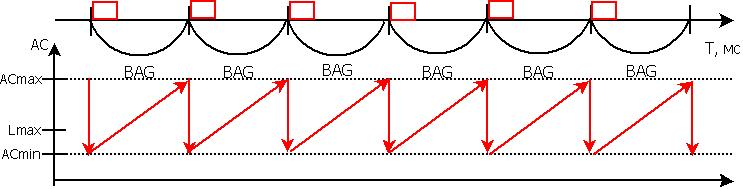
\includegraphics[width=0.80\textwidth]{img/nojit.png}
	\caption[russian]{Работа алгоритма текущего ведра при нулевом джиттере.}
	\label{pic:scheme:nojit}
\end{figure}

\begin{figure}[h!]
	\centering
	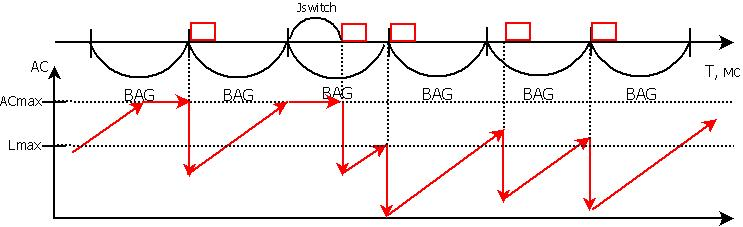
\includegraphics[width=0.80\textwidth]{img/jit.png}
	\caption{Работа алгоритма текущего ведра при ненулевом джиттере.}
	\label{pic:scheme:jit}
\end{figure}

\subsection{Реализации схемы управления трафиком}
В данном разделе описываются индивидуальные особенности следующих схем управления трафиком:
\begin{itemize}
	\item AFDX.
	\item FC-AE-ASM-RT.
	\item Предложенная автором схема управления трафиком в ПКС.
\end{itemize}

Стандарты AFDX и FC-AE-ASM-RT определяют построение сетей ВС РВ на основе виртуальных каналов. Маршрутизация в таких сетях производится коммутаторами при помощи статических таблиц, которые настраиваются заранее. Контроль трафика осуществляется с использованием алгоритма текущего ведра на уровне кадров. Алгоритм встроен в специализированные коммутаторы этих сетей.

В ПКС маршрутизация производится коммутаторами на основе динамических таблиц, задаваемых контроллером. Предложенная автором схема основывается на механизме meter-таблиц \cite{meter}, показанных на рисунке~\ref{pic:scheme:meter} и являющихся частью стандарта OpenFlow1.3 \cite{openflow}. Такие таблицы также управляются контроллером и могут быть изменены в процессе работы системы. Каждая запись meter-таблицы задаёт измеритель, контролирующий скорость привязанных к нему потоков. Схема, по которой осуществляется данный контроль, не закреплена в стандарте и зависит от конкретных реализаций. 

\begin{figure}[h!]
	\centering
	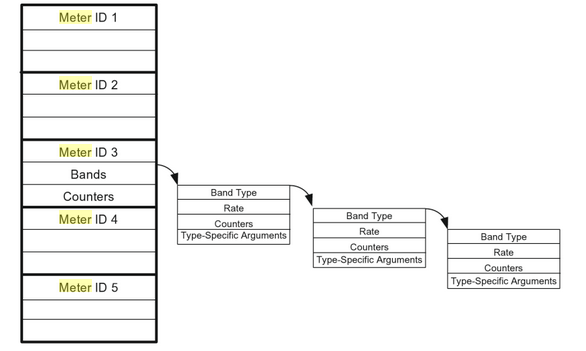
\includegraphics[width=0.80\textwidth]{img/meter.png}
	\caption{Структура meter-таблицы.}
	\label{pic:scheme:meter}
\end{figure}

Программный коммутатор Ofsoftswitch13 \cite{ofsoftswitch} реализует контроль трафика измерителями при помощи алгоритма текущего ведра и поэтому лег в основу схемы управления трафиком в ПКС.

Схема управления трафиком:
\begin{itemize}
	\item Для каждого потока задается свой измеритель, на который средствами OpenFlow, посылается максимальное значение кредита и скорость его роста.
	\item Проверка допустимости трафика производится при помощи алгоритма текущего ведра отдельно для каждого потока на уровне пакетов.
\end{itemize}

\subsection{Сравнение реализаций по критерию поддержки реконфигурируемости}
Конфигурацией сети на основе виртуальных каналов назовем набор параметров виртуальных каналов в совокупности с их маршрутами. Каждой конфигурации соответствует набор таблиц маршрутизации, определяющих действия коммутаторов по передаче данных и контролю трафика в соответствии с данной конфигурацией.

Стандарт AFDX предусматривает наличие одной фиксированной таблицы маршрутизации на каждом коммутаторе. Такой набор таблиц маршрутизации соответствует единственной доступной в сети AFDX конфигурации.

Стандарт FC-AE-ASM-RT имеет возможность поддерживать на коммутаторах несколько таблиц маршрутизации, задаваемых до начала работы системы. Это позволяет задать несколько конфигураций сети. Переход между такими конфигурациями осуществляется при помощи контроллера конфигураций. Им является дополнительная оконечная станция. При смене конфигурации контроллер сообщает коммутаторам сети идентификатор новой конфигурации. На каждом коммутаторе находится внутренняя оконечная станция, обрабатывающая информацию о смене конфигурации. Так как контроллером передается только идентификатор, весь набор конфигураций должен быть заложен в коммутаторы до начала работы системы. На время процесса перехода, который может длиться до 40 мс, все коммуникации в системе временно приостанавливаются, так как происходит полная смена таблиц коммутации. Таким образом процесс смены конфигурации нарушает циркуляцию трафика всех потоков данных системы.

В ПКС таблицы коммутаторов управляются контроллером при помощи сообщений, регламентируемых протоколом OpenFlow. В предложенной автором схеме модификация параметров виртуальных каналов производится сообщениями FlowMod и MeterMod протокола OpenFlow1.3. За счёт этого таблицы маршрутизации, равно как и meter-таблицы, могут быть изменены любым образом в ходе работы системы. Это позволяет создавать множество конфигураций, размер которого ограничен лишь возможностями физической среды передачи данных. Процесс изменения таблиц коммутаций не затрагивает абсолютно все, содержащиеся в них правила. Это даёт возможность не нарушать движение трафика по виртуальным каналам, маршруты которых не проходили через элементы сети, попавшие под сбой. Для виртуальных каналов, пути следования которых были подвержены поломке, имеется возможность сохранить часть пакетов в случае совпадения участков старого и нового маршрутов. 

Динамическая реконфигурация сетей ВСРВ требуется в случаях:
\begin{enumerate}
	\item смены режимов работы;
	\item выхода из строя вычислителей.
\end{enumerate}

Как было показано выше стандарт AFDX не поддерживает реконфигурацию в ходе работы системы. Возможностей же FC-AE-ASM-RT недостаточно для произведения гибкой реконфигурации, так как все сбойные режимы должны быть заранее заложены в у. Для единичного отказа число таких режимов является достаточно большим и оценивается количеством физических элементов сети. Расчет всех случаев множественного отказа является ещё более нетривиальной задачей, а хранение всех таких конфигураций в памяти коммутаторов не представляется возможным. Использование ПКС в ВС РВ позволяет производить расчет и применение новой конфигурации сети непосредственно при возникновении поломки. Такой вариант реконфигурации позволяет системе частично продолжать функционировать даже в процессе перехода. Всё это даёт возможность гибко реагировать на множественные сбои и восстанавливать работу системы в полном объеме в тех случаях, когда это позволяют физические ресурсы.


\section{Актуальность задачи}
Динамическая реконфигурация сети востребована в ВС РВ. Возможность перераспределить потоки данных в ходе работы системы необходима при возникновении сбоев или желании заложить несколько режимов работы в систему.

В разделе \ref{sec:scheme} было продемонстрировано, что в ПКС имеются возможности для гибкой реконфигурации сети при соблюдении требований к качеству обслуживания, принятых в сетях ВС РВ. Для осуществления реконфигурации в случае возникновения сбоев необходимо:
\begin{enumerate}
	\item Определить, в какой части сети произошел сбой.
	\item Произвести расчет новой конфигурации с учетом вышедших из строя элементов сети.
	\item Произвести переход на полученную конфигурацию.
\end{enumerate}

Данная работа посвящена вопросу идентификации сбоев и алгоритму расчета новой конфигурации сети. Процедура смены конфигураций была ранее реализована и апробирована автором на предмет пригодности в рамках подтверждения работоспособности схемы управления трафиком в ПКС.

\section{Алгоритм реконфигурации виртуальных каналов}
\subsection{Общая схема алгоритма}
В условиях реального времени требуется произвести реконфигурацию за как можно
более короткий срок и с минимальными изменениями в сети. Для этого на базовом этапе
рассматриваются только те виртуальные каналы, которые необходимо переложить, так
как они проходят через сбойные элементы сети. В случае если невозможно произвести
реконфигурацию, рассматривая только это множество виртуальных каналов, для
восстановления работы сети производится дополнительный этап, на котором также
затрагиваются не поврежденные виртуальные каналы.
Применение новых маршрутов в сети осуществляется только после успешного
завершения работы алгоритма. Поведение приложения реконфигурации при неуспешном
завершении алгоритма в рамках данной работы не рассматривается. Однако
предполагается, что в этом случае будет предпринята попытка переложить хотя бы часть
виртуальных каналов на основе результатов дополнительного или базового этапов.

\subsection{Процедуры поиска нового маршрута виртуального канала}
Введём обозначения:
( ) – отправитель для данного виртуального канала.
 ( ) – получатель для данного виртуального канала.
(1) – один из узлов, между которыми прервалась связь, ближний к ( ) .
(2) – один из узлов, между которыми прервалась связь, ближний к ( ) .
Предлагается два варианта алгоритма поиска нового маршрута виртуального
канала. На разных этапах алгоритма реконфигурации могут быть использованы разные
варианты. Этот выбор является частью экспериментального исследования.
Первый вариант алгоритма:
1. Используя алгоритм Дейкстры, найти кратчайший путь между (1) и ( ) .
2. Добавить в него путь от ( ) к (1) .
3. Удалить циклы.
Второй вариант алгоритма:
1. Используя алгоритм k-кратчайших путей [11], найти кратчайший путь между ( ) и
( ) .
2. Выбрать путь по критерию совпадения со старым маршрутом.

\subsection{Описание базового этапа алгоритма}
На данном этапе производится попытка найти новые маршруты для виртуальных
каналов, проходивших через сбойные элементы. При этом не затрагиваются остальные
виртуальные каналы. Такой подход при успешном завершении данного этапа позволяет
произвести минимальные изменения в сети.
Обозначим ( ) подмножество всех виртуальных каналов, проходивших через
отказавший коммутатор или физическую линию.Пропускная способность
вычисляется
из параметров виртуального канала.
=
Базовый этап.
1. Для каждого виртуального канала из набора ( ) в порядке убывания пропускной
способности выполнить:
1.1. Удалить все ребра, на которых не хватает пропускной способности для данного
виртуального канала.
1.2. Запустить один из алгоритмов поиска нового маршрута виртуального канала,
указанных в разделе 4.4. В случае неуспеха перейти к пункту 3.
172. Если для всех виртуальных каналов из множества ( ) найдены новые маршруты,
перейти к пункту 3.
3. Завершить этап.

\subsection{Описание дополнительного этапа алгоритма}
На данном этапе задействуется более широкий набор виртуальных каналов, чем на
базовом этапе.
Пусть
– максимальная пропускная способность виртуальных каналов из
множества ( ) .
Обозначим ( ) подмножество всех виртуальных каналов, которые не входят в ( ) и
пропускная способность которых не больше
.
В качестве дополнительного этапа выполнить:
1. Для каждого виртуального канала из набора ( ) в порядке убывания пропускной
способности выполнить:
1.1. Удалить все ребра, на которых не хватает пропускной способности для данного
виртуального канала.
1.2. Запустить один из алгоритмов поиска нового маршрута виртуального канала,
указанных в разделе 4.4. В случае неуспеха перейти к пункту 2.
2. Для каждого виртуального канала из набора ( ) в порядке убывания пропускной
способности выполнить:
2.1. Удалить все ребра, на которых не хватает пропускной способности для данного
виртуального канала.
2.2. Запустить второй вариант алгоритма поиска нового маршрута виртуального
канала, описанный в разделе 4.4. В случае неуспеха перейти к пункту 2.
3. Завершить этап.


\section{Структура и функции приложения реконфигурации}
\subsection{Структура приложения реконфигурации}


\subsection{Описание функций служебной части}
Служебная часть должна предоставляет управляющей:
\begin{itemize}
	\item информацию о потоках данных, которыми обмениваются абоненты сети;
	\item информацию о проложенных в сети виртуальных каналах и их параметрах;
	\item интерфейс для добавления/удаления/модификации виртуальных каналов с определенными параметрами качества обслуживания.
\end{itemize}

\subsection{Описание функций управляющей части}
Управляющая часть:
\begin{itemize}
	\item отвечает за построение маршрутов виртуальных каналов;
	\item отвечает за построение новых маршрутов виртуальных каналов при выходе из строя компонентов сети;
	\item использует API служебной части для применения новых маршрутов в сети после завершения работы алгоритма реконфигурации;
	\item использует информацию, полученную от монитора, для инициализации алгоритма реконфигурации.
\end{itemize}
\subsection{Описание функций монитора}
Монитор сети:
\begin{itemize}
	\item отвечает за построение начальной топологии сети;
	\item сообщает управляющей части о выходе из строя компонентов сети.
\end{itemize}


\section{Программная реализация}
\subsection{Выбор базового программного обеспечения сети}
\subsection{Структура программного средства}

Основные программные компоненты служебной части:
\begin{itemize}
	\item Sla - класс характеристик виртуальных каналов.
	\item Vl - класс, отвечающий за хранение параметров виртуальных каналов (включая их маршруты). Также формирует набор сообщений для применения соответствующих параметров в сети.
	\item VlSet - набор виртуальных каналов.
\end{itemize}

Основные программные компоненты управляющей части:
\begin{itemize}
	\item Netcontrol - класс, отвечающий за запуск алгоритма реконфигурации. Является классом приложения Runos.
	\item Algorithm - класс, реализующий алгоритмы построения маршрутов виртуальных каналов.
\end{itemize}


Основные программные компоненты монитора:
\begin{itemize}
	\item NetTopology - класс, отображающий текущее состояние топологии сети. Использует вспомогательные классы NetLink, NetSwitch и NetHost для хранения информации о каналах, коммутаторах и абонентах соответственно.
	\item BandwidthInfo - хранит текущую доступную на физических каналах пропускную способность. Начальные значения задаются в конфигурации приложения.
	\item HostManager - приложение Runos, анализирующее состояние абонентов. Приложение написано автором работы.
	\item SwitchManager - приложение Runos, анализирующее состояние коммутаторов. Используется стандартное приложение, входящее в состав контроллера.
	\item LinkDiscovery - приложение Runos, анализирующее состояние физических каналов. Используется стандартное приложение, входящее в состав контроллера.
\end{itemize}


\section{Экспериментальное исследование}
\subsection{Цель исследования}
Целью исследования является подтверждение характеристик предложенного в работе алгоритма реконфигурации виртуальных каналов, предназначенного для использования в рамках описанного подхода к передаче данных в ПКС в условиях реального времени. Для достижения поставленной цели необходимо:
\begin{itemize}
	\item провести исследование свойств алгоритма на различных классах входных данных; 
	\item провести апробацию работы алгоритма в составе приложения, реализующего функции реконфигурации и мониторинга.
\end{itemize}

Свойства алгоритма, подлежащие исследованию:
\begin{itemize}
	\item успешность и этап завершения;
	\item скорость работы.
\end{itemize}

Изучаемые в рамках апробации подхода характеристики системы:
\begin{itemize}
	\item успешность восстановления трафика в сети после завершения работы алгоритма реконфигурации;
	\item скорость применения изменений в сети;
	\item характеристики качества обслуживания для трафика абонентов (задержка и джиттер).
\end{itemize}

\subsection{Классы исходных данных}
Параметры для формирования классов данных:
\begin{enumerate}
	\item Распределение каналов по пропускным способностям.
	\item Общая загруженность сети.
	\item Топология сети.
\end{enumerate}

Расчёт пропускной способности виртуального канала производится в соответствии с формулой:
$$bw = \frac{LM}{BAG}$$

Выделим типы виртуальных каналов в зависимости от пропускной способности:
\begin{itemize}
	\item легковесные ($bw=k$);
	\item средние ($bw=2k$);
	\item тяжёлые ($bw=4k$).
\end{itemize}

Классы исходных данных, сформированные на основе процентного содержания виртуальных каналов каждого типа, показаны в таблице~\ref{table:bwclass}. Данные классы выбраны для исследования случаев преобладания каждого из типов виртуальных каналов. Распределение пропускных способностей входных потоков данных влияет на работу алгоритма, так как поиск альтернативного маршрута виртуальных каналов затрудняется с ростом их пропускной способности.

\begin{table}[h]
\begin{center}
\begin{tabular}{|c|c|c|c|}
\hline
	 & Легковесные & Средние & Тяжёлые\\
\hline
	1 & 90\% & 7\% & 3\% \\
\hline
 2 & 10\% & 80\% & 10\% \\
\hline
	3 & 33\% & 34\% & 33\% \\
\hline
	4 & 5\% & 15\% & 80\% \\
\hline
\end{tabular}
\end{center}
\caption{Классы данных на основе пропускной способности}
\label{table:bwclass}
\end{table}

Расчёт общей загруженности сети производится при помощи формулы, отражающей утилизацию физических линий в зависимости от количества маршрутов виртуальных каналов, которые могут быть проложены через данную линию.

Для графа сети, в котором ребра соответствуют физическим линиям, введём вес ребра $e$:
$$p_{e} = \sum_{vl}\frac{bw_{vl} \ast k_{vl_e}}{k_{vl}}$$
где 
\begin{itemize}
	\item $vl$ -- множество виртуальных каналов;
	\item $bw_{vl}$ -- пропускная способность виртуального канала;
	\item $k_{vl_e}$ -- число кратчайших путей, построенных для данного канала, проходящих через это ребро;
	\item $k_{vl}$ -- количество найденных кратчайших путей для данного виртуального канала.
\end{itemize}

Тогда общая загруженность сети определяется формулой:
$$p = \max_{e}\frac{p_{e}}{bw_{e}}$$

где $bw_{e}$ -- пропускная способность физической линии.

Два класса исходных данных, формирующиеся на основе данного параметра, показаны в таблице~\ref{table:loadclass}. Общая загруженность сети влияет на работу исследуемого алгоритма. С ростом загруженности возрастает сложность поиска альтернативных маршрутов для виртуальных каналов. 

\begin{table}[h]
\begin{center}
\begin{tabular}{|c|c|}
\hline
	& Загруженность сети ($p$)\\
\hline
	1 & 60\% \\
\hline
	2 & 80\% \\
\hline
\end{tabular}
\end{center}
\caption{Классы данных на основе загруженности сети}
\label{table:loadclass}`
\end{table}

Для апробации выхода из строя различных элементов сети и демонстрации множества вариантов поиска альтернативного маршрута было выбрано три топологии:
\begin{enumerate}
	\item <<Ромб>> (Рис.~\ref{pic:4node}).
	\item <<Двойное резервирование>> (Рис.~\ref{pic:double}).
	\item <<add Название>> (Рис.~\ref{pic:5node}).
\end{enumerate}

\begin{figure}[h!]
	\centering
	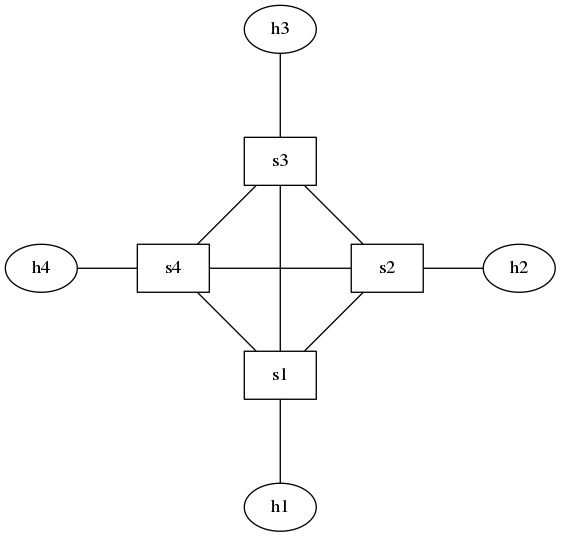
\includegraphics[width=0.40\textwidth]{img/4node.png}
	\caption{Топология <<Ромб>>.}
	\label{pic:4node}
\end{figure}

\begin{figure}[h!]
	\centering
	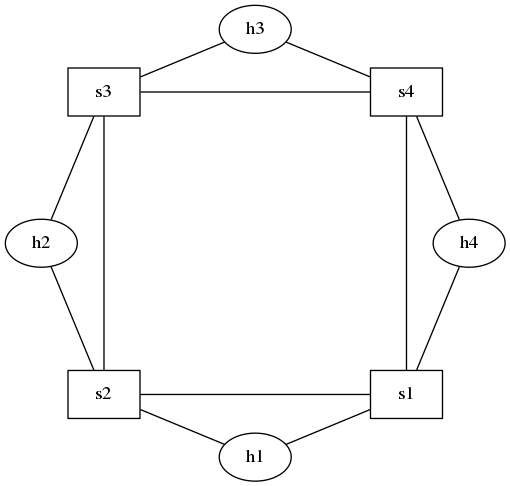
\includegraphics[width=0.40\textwidth]{img/double.png}
	\caption[russian]{Топология <<Двойное резервирование>>.}
	\label{pic:double}
\end{figure}

\begin{figure}[h!]
	\centering
	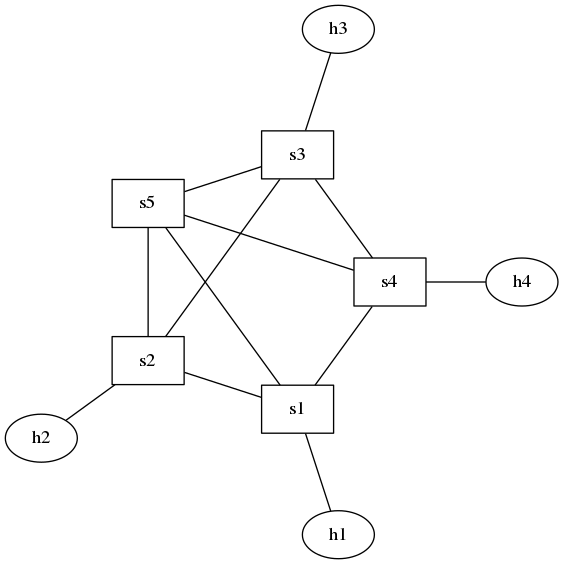
\includegraphics[width=0.40\textwidth]{img/5node.png}
	\caption{Топология <<add Название>>.}
	\label{pic:5node}
\end{figure}

В исследовании используется рекомендованное экспертами в области вычислительных реального времени число потоков данных равное 100.

\subsection{Накладываемые ограничения} \label{subsec:limits}
Процесс реконфигурации сети влечёт за собой потери пакетов, увеличение задержек и джиттеров. Чем быстрее будет производится смена конфигурации, тем меньше эффекта этот процесс окажет на трафик абонентов бортовой системы. В рамках данного экспериментального исследования будем опираться на временные ограничения, принятые в вычислительных системах реального времени. Как упоминалось в разделе~\ref{sec:scheme}, в сетях FC-AE-ASM-RT на смену конфигурации отводится 40мс. При этом будем учитывать оценки на время, прошедшее с момента отправки последнего управляющего правила до момента его применения в таблице коммутации:

С учётом вышесказанного в качестве итогового времени, отводимого на реконфигурацию примем addмс.
\subsection{Исследование свойств алгоритма}
\subsubsection{Методика исследования}
Исследование свойств алгоритма производится по следующей схеме:
\begin{enumerate}
	\item Для каждого класса данных генерируется соответствующий ему набор виртуальных каналов.
	\item Для каждого набора виртуальных каналов:
	\begin{enumerate}
		\item Запускается приложение, содержащее алгоритм реконфигурации.
		\item Запуск инициирует построение начальных маршрутов виртуальных каналов.
		\item Собирается статистика по количеству виртуальных каналов, проходящих через каждый элемент сети.
		\item Выбирается элемент сети, через который проходит наибольшее число виртуальных каналов, и имитируется его поломка.
		\item Поломка инициирует запуск алгоритма реконфигурации.
		\item По завершению алгоритм выдаёт информацию об успешности и этапе завершения, а так же времени работы.
	\end{enumerate}
	\item Предполагается, что время работы алгоритма занимает не более 70\% от всего времени, заложенного на реконфигурацию.
	\item По полученным характеристикам делается вывод о возможности использования алгоритма в рамках подхода к передаче данных в реальном времени.
\end{enumerate}
 
\subsubsection{Результаты}
Характеристики компьютера, на котором производилось исследование:
\begin{itemize}
	\item Процессор -- Intel Core i7, тактовая частота 1.90 ГГц.
	\item Оперативная память -- 4 ГБ.
\end{itemize}

Результаты исследования свойств алгоритма реконфигурации виртуальных каналов приведены в addПриложение (см. таблицу addТаблица).

Максимальное время работы алгоритма – addмс. Данные показатели времени достигаются, если алгоритм вынужден выполнить дополнительный этап. Следует отметить, что выполнение дополнительного этапа произошло в add\% случаев. Как правило алгоритм завершает работу на базовом этапе. При таком варианте выполнения время завершения алгоритма не превышает addмс. Время работы алгоритма, не превысило 70\% от времени, отведённого на реконфигурацию. То, как данная величина соотносится со временем, затрачиваемым на применение полученных изменений в сети, будет продемонстрировано в разделе~\ref{subsec:approbation}.

Алгоритм не смог построить новую систему виртуальных каналов при add. Это объясняется тем, что add.

\subsection{Апробация разработанного подхода динамической реконфигурации сети} \label{subsec:approbation}
\subsubsection{Конфигурация экспериментальной системы}
Система апробации представляет собой виртуальную среду, имитирующую
функционирование:
\begin{enumerate}
	\item Контроллера сети.
	\item Набора коммутаторов.
	\item Абонентов сети, формирующих потоки данных с заданными характеристиками.
\end{enumerate}

Виртуальная среда разворачивается на основе операционной системы Ubuntu 16.04,
на которой установлены следующие компоненты:
\begin{enumerate}
	\item Runos -- ПКС-контроллер \cite{runos}.
	\item Ofsoftswitch13 -- программный коммутатор, поддерживающий OpenFlow 1.3 \cite{ofsoftswitch}.
	\item Mininet -- средство имитирующее работу сети \cite{mininet}.
\end{enumerate}

\subsubsection{Сценарии апробации}

Для апробации предложенного подхода к передаче данных в реальном времени был выбран набор сценариев, основывающийся на том, какие элементы сети могут выйти из строя. 

Рассматривается выход из строя:
\begin{enumerate}
	\item Коммутатора.
	\item Физической линии, соединяющей два коммутатора.
	\item Физической линии, соединяющей абонента с коммутатором.
	\item Порта абонента или коммутатора.
\end{enumerate}

Дополнительно к этому рассматриваются сценарии кратных последовательных во времени выходов из строя элементов сети.

Сценарии разрыва физической линии между коммутаторами и выхода из строя соответствующих портов производятся на всех топологиях. Оставшиеся сценарии могут быть выполнены только на топологиях <<Двойное резервирование>> и <<add Название>> (см. Рис.~\ref{pic:double} и Рис.~\ref{pic:5node}).

\subsubsection{Методика апробации}
Апробация работы алгоритма реконфигурации в рамках предложенного подхода состоит из трёх этапов:
\begin{enumerate}
	\item Формирование набора тестовых прецедентов.
	\item Проведение экспериментов на тестовых прецедентах.
	\item Анализ результатов.
\end{enumerate}

Тестовые прецеденты формируются выбором:
\begin{itemize}
	\item сценария апробации;
	\item класса исходных данных с доступной для выбранного сценария топологией сети.
\end{itemize}

На этапе проведения экспериментов производится запуск каждого тестового прецедента:
\begin{enumerate}
	\item Формируется соответствующая классу данных конфигурация сети.
	\item Запускается приложение реконфигурации.
	\item Запускается виртуальная тестовая среда, имитирующая поведение сети.
	\item Запуск приложения инициирует построение начальных маршрутов виртуальных каналов.
	\item Запуск тестовой среды инициирует отправку и прием потоков данных абонентами, а так же сбор статистики по этим потокам данных.
	\item Средствами тестовой среды запускается сценарий апробации.
	\item Соответствующая сценарию поломка инициирует запуск алгоритма реконфигурации.
	\item По завершению алгоритм выдаёт информацию о времени, затраченном на применение изменений в сети.
	\item Происходит сворачивание тестовой среды, инициирующее обработку собранной статистики по потокам данных.
\end{enumerate}

На этапе анализа результатов для каждого тестового прецедента:
\begin{enumerate}
	\item Проверяется факт восстановления трафика по завершению выполнения сценария.
	\item Анализируется время, затраченное на применение изменений в сети.
	\item Анализируется число потерянных в ходе реконфигурации пакетов.
	\item Задержки и джиттеры, полученные в период реконфигурации сравниваются с эталонными задержками, полученными в штатном режиме.
	\item Делается вывод об успешности работы приложения реконфигурации в рамках предложенного сценария.
\end{enumerate}

\subsubsection{Результаты}

Результаты апробации работы алгоритма в рамках приложения, реализующего подход к передаче данных в условиях реального времени в ПКС, приведены в addПриложение (см. таблицу addТаблица).

Джиттеры и задержки потоков данных, виртуальные каналы которых участвовали в реконфигурации, отличались от эталонных не более, чем на addмс и addмс соответственно. Данное отклонение лежит в рамках допустимого. Джиттеры и задержки прочих потоков данных не изменились.

Максимальное время затраченное на процесс реконфигурации удовлетворяет наложенным в разделе~\ref{subsec:limits} ограничениям. Потери пакетов составили add. При этом потоки, маршруты виртуальных каналов которых не проходили через сбойные элементы, затронуты не были.

Отказы от построения новых виртуальных каналов были получены на тех же классах данных, что и при исследовании свойств алгоритма.

Было проверено несколько сценариев кратного последовательного во времени выхода из строя элементов сети. Максимальное число последовательных поломок, после которых восстанавливалась работоспособность системы, составило add. Отказы от восстановления работы сети после очередной поломки были обусловлены исключительно отсутствием путей между абонентами или нехваткой пропускных способностей.

\subsection{Выводы}
Проведенное экспериментальное исследование продемонстрировало, что:
\begin{itemize}
	\item основные характеристики алгоритма соответствуют ожидаемым;
	\item алгоритм успешно функционирует в рамках приложения реконфигурации, работающего в виртуальной среде, имитирующей сеть ПКС;
	\item соблюдаются ограничения на характеристики качества обслуживания абонентских потоков данных при реконфигурации сети с использованием предложенного алгоритма.
\end{itemize}

Исследование и апробация показали, что предложенный алгоритм реконфигурации виртуальных каналов способен работать в составе приложения, реализующего подход к передаче данных в реальном времени в ПКС. Алгоритм успешно осуществляет поиск новых маршрутов для виртуальных каналов при выходе из строя различных элементов сети. Апробация показала работоспособность разработанного приложения, осуществляющего функции реконфигурации и мониторинга, и реализуемого им подхода. Время, затраченное на осуществление реконфигурации, не превосходит ограничений, заданных в существующих системах реального времени.

\section*{Заключение}
\addcontentsline{toc}{section}{Заключение}
текст

\renewcommand{\bibname}{Список литературы}
\addcontentsline{toc}{section}{\bibname}
\bibliographystyle{unsrt}
\begin{thebibliography}{}
	\bibitem{afdx}
	AFDX / ARINC 664 Tutorial (1500-049) // Condor Engineering, Inc. -- 2005.
	\bibitem{fcaert}
	Fibre Channel Arbitrated Loop (FC-AL) // working draft proposal American National Standard for Information Technology. 1995. 98 p.
	\bibitem{sdn}
	Software-Defined Networking: The New Norm for Networks // Open Networking Foundation. -- 2012. [PDF] (https://www.opennetworking.org/images/stories/downloads/sdn-resources/white-papers/wp-sdn-newnorm.pdf)
	\bibitem{meter}
	Efimushkin, T. Ledovskikh, D. Korabelnikov, D. Iazykov. Perfomance assurance in Software-Defined Networks // « Intellect Telecom» JSC.
	\bibitem{openflow}
	ONF OpenFlow Switch Specification, Version1.3.0 [PDF] (https://www.opennetworking.org/images/stories/downloads/sdn-resources/onf-specifications/openflow/openflow-spec-v1.3.0.pdf)
	\bibitem{ofsoftswitch}
	CPqD F. Openflow 1.3 software switch [HTML] (http://www.cpqd.github.io/ofsoftswitch13/).
	\bibitem{runos}
	Shalimov A. et al. The Runos OpenFlow Controller // Software Defined Networks (EWSDN), 2015 Fourth European Workshop on. -- IEEE, 2015. -- С. 103-104.
	\bibitem{mininet}
	Oliveira R. L. S. Using mininet for emulation and prototyping software-defined networks // Communications and Computing (COLCOM) -- 2014. -- P. 1-6
\end{thebibliography}

\end{document}